\documentclass[11pt, a4paper]{article}
\usepackage[margin=1cm]{geometry}
\parindent 0px % indent new lines by 0 pixels
\usepackage[utf8]{inputenc}
\usepackage{hyperref, amsfonts,amssymb,amsmath,tikz,pgfplots,float,graphicx}
\usetikzlibrary{positioning}

\title{\small AS91522 - Physics 3.2\\ \huge Circular Motion of a Stunt Glider}
\author{Nathan Tasker}
\date{\today}

\begin{document}
	\maketitle
	\tableofcontents
	\newpage
	\section{Vertical Circle: Loop the loop including Dip and Arch}
	\subsection{Achieved}
	During motion, 3 forces are acting on the stunt glider:
	\begin{enumerate}
		\item Gravity ($\vec{F_g}$) (i.e. Weight) always vertically downwards (i.e. toward center of Earth).
		\item Lift ($\vec{F_L}$) perpendicular to direction of velocity, toward the center of the circular path.
		\item Air Resistance ($\vec{F_R}$) (i.e. Friction, Drag) opposite to direction of velocity.
	\end{enumerate}
	Please note that vector arrow lengths are not perfectly proportionally accurate.
	\begin{center}
		\begin{tikzpicture}
			\pgfmathsetmacro{\MaxVelocityLength}{2}
			\pgfmathsetmacro{\MinVelocityLength}{1}
			\pgfmathsetmacro{\MaxResistanceLength}{\MaxVelocityLength*0.5}
			\pgfmathsetmacro{\MinResistanceLength}{\MinVelocityLength*0.5}
			\pgfmathsetmacro{\GravityLength}{1}
			\pgfmathsetmacro{\PathRadius}{5}
			\pgfmathsetmacro{\GliderPointRadius}{0.1}
			\coordinate(TopPos) at (0,\PathRadius);
			\coordinate(BottomPos) at (0,-\PathRadius);
			
			\draw[dashed, gray] (0,0) circle (\PathRadius);
			
			\filldraw[black] (TopPos) circle (\GliderPointRadius);
			\draw[->] (TopPos) -- ++(-\MinVelocityLength,0) node[left] {$\vec{v}$};
			\draw[->] (TopPos) -- ++(0,-\GravityLength) node[below] {$\vec{F_g}$};
			\draw[->] (TopPos) -- ++(0,-0.5) node[right] {$\vec{F_L}$};
			\draw[->] (TopPos) -- ++(\MinResistanceLength,0) node[right] {$\vec{F_R}$};
			
			\filldraw[black] (BottomPos) circle (\GliderPointRadius);
			\draw[->] (BottomPos) -- ++(\MaxVelocityLength,0) node[right] {$\vec{v}$};
			\draw[->] (BottomPos) -- ++(0,-\GravityLength) node[below] {$\vec{F_g}$};
			\draw[->] (BottomPos) -- ++(0,2) node[above] {$\vec{F_L}$};
			\draw[->] (BottomPos) -- ++(-\MaxResistanceLength,0) node[left] {$\vec{F_R}$};
		\end{tikzpicture}
	\end{center}
	The force of gravity is always constant in both magnitude and direction regardless of the glider's velocity or position in the loop (top, bottom, and anywhere else). This is because $|\vec{F_g}|=mg$ where mass ($m$) and the acceleration of gravity ($g$) are constants.\\
	Conversely, the force of lift varies in both direction and magnitude as the glider performs the loop the loop.\\
	Lift's magnitude ($|\vec{F_L}|$) is greatest at the bottom, $\because |\vec{F_L}|=\frac{1}{2}pv^2AC_L$, $\therefore |\vec{F_L}|\propto v^2$. Because velocity is greatest at bottom, lift force is as well. To maintain circular motion the centripetal force ($|\vec{F_c}|=|\vec{F_L}|-|\vec{F_g}|$) towards the center of the circular path must have a magnitude value great enough to provide necessary centripetal acceleration for the circular path radius, meaning the lift force upwards must at least be greater than the gravity force downwards ($|\vec{F_L}|>|\vec{F_g}|$ in order for $|\vec{F_c}|>0$).\\
	Lift's magnitude ($|\vec{F_L}|$) is least at the top, because the direction of gravity force is toward the center of the circular path. This means ($|\vec{F_c}|=|\vec{F_L}|+|\vec{F_g}|$).\\
	\begin{center}
		\begin{tikzpicture}
			\pgfmathsetmacro{\HalfWidth}{8};
			\pgfmathsetmacro{\TopLineY}{3.05};
			\pgfmathsetmacro{\BottomLineY}{-2.65};
			%\coordinate(TopPos) at (0,\PathRadius);
			%\coordinate(BottomPos) at (0,-\PathRadius);
			\node[inner sep=0] at (0,0) {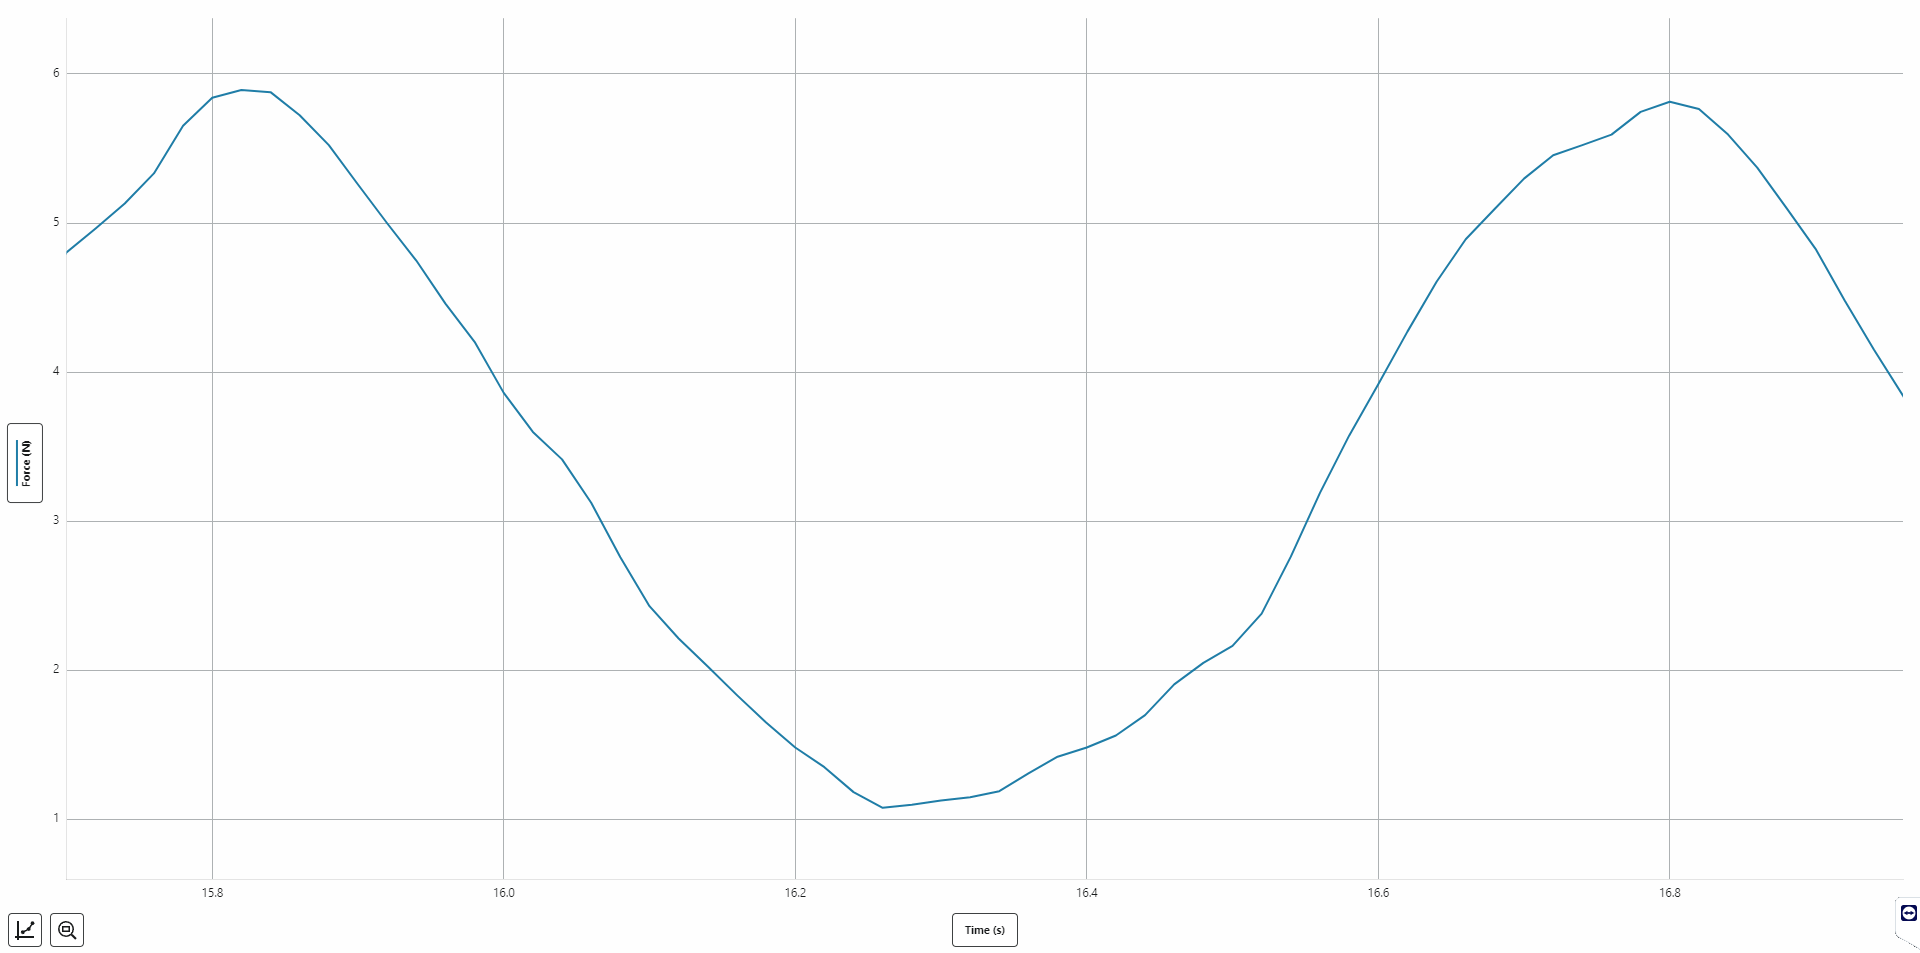
\includegraphics[width=0.8\textwidth]{Images/Loop the loop graph.png}};sdfsdfsdfsdfsfd
			\draw[gray, dashed] (-\HalfWidth,\TopLineY) -- (\HalfWidth,\TopLineY);
			\draw[gray, dashed] (-\HalfWidth,\BottomLineY) -- (\HalfWidth,\BottomLineY);
		\end{tikzpicture}
	\end{center}
	At the bottom of the vertical circle, the tension force (emulating the lift force, $\vec{F_L}$) is greatest, which occurs at 15.82 seconds with 5.89N.\\
	Once the force meter (emulating motion of glider) reaches the top of the verticle circle, the tension force is at its least, which - when smoothing the curve of data and reducing random variation/noise - occurs at\\
	Check if sine model helps then return to this section.\\
	During the loop the loop, as the glider ascends, its kinetic energy ($E_K$) is converted into gravitational potential energy ($E_p$). As the glider descends, its gravitational potential energy ($E_p$) is converted back into kinetic energy ($E_K$).
	
	\subsection{Merit}
	\subsection{Excellence}
	\section{Banked Corner}
	\subsection{Achieved}
	\subsection{Merit}
	\subsection{Excellence}
	\section{Additional Info}
	\subsection{Comprehensive Version History}
	Access to all prior versions of this document during process of creation is publicly available at:\\
	\url{https://github.com/NathanTaskerPersonal/AS91522}
	\subsection{Graphical Analysis Files}
	Access to all graphical analysis files are publically available at:\\
	\href{https://middletonschoolnz-my.sharepoint.com/:f:/g/personal/taskern_middleton_school_nz/EhEmw21C2L9Fn9BYUy2ccwMBn6xCUF93vtfvtT_5_rkxbA?e=Tp02lP}{middletonschoolnz-my.sharepoint.com/...}
	\subsection{Bibliography}
\end{document}
